% Supplemental Material.
% Values transcribed from results/*.json; see docs/ for the narrative versions.
\documentclass[aps,prd,onecolumn,superscriptaddress,nofootinbib]{revtex4-2}

\usepackage{amsmath,amssymb,amsthm,graphicx,hyperref,booktabs,float}

\newcommand{\TODO}[1]{\textbf{[#1]}}
\newcommand{\Rem}{\mathrm{Re}}
\newcommand{\Imm}{\mathrm{Im}}
\newcommand{\Ord}{\mathcal{O}}
\renewcommand{\thesection}{S\arabic{section}}
\renewcommand{\thetable}{S\Roman{table}}
\renewcommand{\thefigure}{S\arabic{figure}}
\renewcommand{\theequation}{S\arabic{equation}}

\begin{document}

\title{Supplemental Material:\\
Symmetry control of exceptional structure in the massive scalar quasinormal
spectrum of doubly rotating five-dimensional Myers--Perry black holes}

\author{\TODO{author names not assigned}}
\affiliation{\TODO{affiliation not assigned}}

\date{\today}
\maketitle

%-------------------------------------------------------------------------
\section{Solvers and their validated domains}\label{sec:solvers}
%-------------------------------------------------------------------------

$r_-$ is the inner horizon radius; $z_-=r_-^2$. Extremality is
$M-(|a|+|b|)^2$, zero at extremality. The independence rule is that any claim
requires agreement between one recurrence solver and one recurrence-free
solver; two wrappers around one discretization do not count.

\begin{table}[H]
\centering\small
\begin{tabular}{llcp{3.1cm}p{4.6cm}}
\toprule
Solver & Formulation & Rec.-free & Validated domain & Known failure \\
\midrule
A & Leaver continued fraction, Gaussian-reduced & no &
  $r_-\le0.2287$, extremality $\ge0.294$ &
  drifts $2$--$6\times10^{-4}$ per depth doubling in the quasiresonant regime \\
B & raw recurrence, Hill determinant, Wynn & no & as A &
  shares A's recurrence; not independent of A \\
C & exterior complex-scaled Chebyshev collocation & yes &
  as A, provided $\theta_{\min}<90^\circ$ &
  no admissible contour as $\Rem\,\Omega\to0$ \\
D & multidomain near-horizon spectral & yes & ordinary modes &
  same formulation limit as C \\
HP & full \texttt{mpmath} chain incl.\ coefficients & no &
  arbitrary precision & slow \\
\bottomrule
\end{tabular}
\caption{Solver inventory. Solver~C's independence is enforced structurally: a
test greps the module for the recurrence routines and fails if any appears.}
\end{table}

The raw Frobenius recurrence has width $13$ for generic two-spin parameters and
$9$ in the static case; the reduction to three terms is exact. The leading
large-$n$ tail is $R_n = 1 + u_1 n^{-1/2}+\dots$ with $u_1=-\sqrt{-2c}$,
$c=i\Omega(r_+-r_-)$, which reduces the required depth by a factor
$\approx1.35$. Higher tail orders are not available: the Gaussian reduction
degrades past $n\sim500$--$800$, where the backward ratio recursion collapses to
a spurious, problem-independent $R_n-1=2/n$.

%-------------------------------------------------------------------------
\section{Benchmarks}\label{sec:bench}
%-------------------------------------------------------------------------

The five-dimensional Schwarzschild--Tangherlini fundamental scalar mode is
reproduced to all $12$ published digits,
\begin{equation}
  \omega = 0.533835574268 - 0.383375368513\,i \qquad (r_+=1),
\end{equation}
with absolute error $5.0\times10^{-13}$ against the published value and
$2.2\times10^{-12}$ between Solvers~A and~B. Four static benchmarks
($\ell=0,1$; $n=0,1$) agree to $10^{-13}$--$10^{-11}$. Three two-spin points
from the literature are reproduced, and the exchange symmetry
$(a,m_1)\leftrightarrow(b,m_2)$ holds numerically to $4.2\times10^{-15}$.
Three solvers agree below $10^{-5}$ on $10/10$ benchmark points.

%-------------------------------------------------------------------------
\section{Atlas census}\label{sec:atlas}
%-------------------------------------------------------------------------

\begin{table}[H]
\centering
\begin{tabular}{lr}
\toprule
Quantity & Value \\
\midrule
atlas points & $50\,558$ \\
independent sectors & $7$ \\
angular branches per sector & $3$ \quad ($\ell_{\min}$, $+2$, $+4$) \\
overtones & $N=0,1,2,3$ \\
parameter points with $\ge2$ branches & $4459$ \\
maximum continued-fraction residual & $3.6\times10^{-9}$ \\
predictor-miss events (recorded, not filled) & $118$ \\
non-convergence events (recorded) & $33$ \\
branch-label collapses excluded & $4$ \\
\bottomrule
\end{tabular}
\caption{Branch atlas census. The atlas itself ($\approx24$~MB) is regenerated
by a deterministic driver and verified against a per-shard SHA-256 manifest
rather than being distributed.}
\end{table}

%-------------------------------------------------------------------------
\section{Diagnostics and the verification gate}\label{sec:gate}
%-------------------------------------------------------------------------

Each gate condition names the routine implementing it; each routine is
validated on closed-form synthetic problems, including negative controls in
which the detector must \emph{not} fire.

\begin{table}[H]
\centering\small
\begin{tabular}{clp{7.0cm}l}
\toprule
& Condition & Synthetic validation & Ten tightest candidates \\
\midrule
G1 & $|a_1/a_2|\to0$ under refinement &
  recovers true separation to $10^{-6}$; invariant under $F\to10^7e^{3z}F$ &
  \textbf{fail} \\
G2 & argument-principle zero count $=2$ &
  counts zeros and poles; raises when unresolved & pass \\
G3 & both roots located without a guess &
  finds both roots of a pair separated by $10^{-3}$ & pass \\
G4 & monodromy transposes the branches &
  swaps for $\lambda^2-t$; \emph{does not} swap for $\lambda^2-(t^2+g^2)$ &
  \textbf{fail} \\
G5 & two loops restore the assignment & verified & --- \\
G6 & splitting $\sim t^{1/2}$, preferred over $t^1$ &
  exponent $0.5\pm10^{-6}$; rejects sqrt for linear splitting &
  \textbf{fail} \\
G7 & Jordan chain solvable, geometric $<$ algebraic &
  fires on a Jordan block; silent on semisimple and block-diagonal & --- \\
G8 & stable under resolution/depth/precision & solver level & --- \\
G9 & confirmed by a recurrence-free solver & cross-solver & --- \\
G10 & inside the validated solver domain & domain guard & pass \\
\bottomrule
\end{tabular}
\caption{The EP2 gate. G2 and G3 are \emph{preconditions}: they establish only
that two distinct roots sit near each other. The decisive evidence is G1, G4
and G6, which fail uniformly, giving the classification ``avoided crossing''.}
\end{table}

An EP3 additionally requires three coalescing branches, zero count $3$,
$a_1=a_2=0$ with $a_3\ne0$, cube-root splitting, a three-cycle monodromy with no
fixed point, and Jordan-chain length $3$.

%-------------------------------------------------------------------------
\section{Certification scope}\label{sec:cert}
%-------------------------------------------------------------------------

Certification claims must name the object certified. We use the labels:
\emph{arithmetic enclosed} (a ball enclosing the value of a given finite
expression); \emph{algebraic-system certified} (a Krawczyk certificate for a
finite-dimensional nonlinear system); \emph{truncated-recurrence certified} (the
above with truncation error bounded); and \emph{continuum certified} (a
statement about the differential operator). Mandatory error separation:
\begin{equation}
  E_{\rm total}\le E_{\rm discretization}+E_{\rm truncation}
  +E_{\rm arithmetic}+E_{\rm root}.
\end{equation}

What is achieved: a Krawczyk existence/uniqueness test (validated in both
directions --- certifying a unique root, excluding a root-free box, and
reporting ``inconclusive'' rather than guessing on an over-large box; it rejects
a midpoint-only Jacobian, which is a heuristic rather than a certificate), and
an Arb ball enclosure of the angular eigenvalue of the $N$-truncated Jacobi
matrix, validated by recovering the exact value $\ell(\ell+2)$ at $c^2=0$.

What is \emph{not} achieved, and why: the radial problem is not certified. The
polynomial coefficients of the recurrence are obtained by a discrete Fourier
transform on a circle, and we have no rigorous bound on its aliasing error, so
$E_{\rm truncation}$ cannot be bounded. This is the exact obstruction, and it is
the reason no truncated-recurrence certificate is claimed anywhere. Closing it
requires either a rigorous aliasing bound or an exact symbolic route to the
coefficients that ball arithmetic can enclose end to end.

%-------------------------------------------------------------------------
\section{Failed approaches, preserved}\label{sec:failed}
%-------------------------------------------------------------------------

Two branch-tracking defects each produced a small computed gap that looked
physical. Both are recorded because the lesson generalizes: \emph{a small
computed gap between two labels is evidence about the labels before it is
evidence about the physics}.

\paragraph*{Branch-label collapse.} With a coarse first step in $s$, the
extrapolator has only one history point and degenerates to the trivial
predictor. A strongly damped $\ell=6$, $N=3$ overtone was captured by the $N=2$
branch while retaining its label, and the tier-1 search reported a minimum gap
of $4.3\times10^{-15}$ at $200$ parameter points. It was caught by the
rescaling-invariant diagnostic, which reported a separation of $\approx1.0$ at
those same points --- a flat contradiction, since a genuine coalescence requires
both to be small. Fixed by finer early steps and a permanent collapse guard.

\paragraph*{Branch jump admitted by a $|\omega|$-relative tolerance.} A
tolerance $\propto|\omega|$ is a constant, and at $|\omega|\approx3.7$ it
admitted a jump in which $\Imm\,\omega$ \emph{reversed} from $-2.530$ to
$-2.762$. The contaminated point was the reported tightest candidate. Fixed by
taking the tolerance from the branch's own history of predictor misses,
$\text{allowed}=\max(4\,\mathrm{median}(\text{prior misses}),\,
0.02\max(|\omega|,1))$, and by reducing the $s$ step to $\le0.05$; an
$\le0.05$ and an $\le0.04$ grid then give identical endpoints on all four
hardest branches.

\paragraph*{A withdrawn bound.} An earlier exclusion in this project used
$\min|dF/d\omega|=1.02\times10^{-2}$. It is withdrawn: $|dF/d\omega|$ is not
invariant under rescaling of the spectral condition. The conclusion survived
re-derivation with invariant quantities; the reasoning did not.

\paragraph*{A misdiagnosed regime.} The failure of the recurrence-free solvers
at large spin was attributed to near-extremality. It is not: ordinary modes
continue to extremality $0.0103$ with residuals $\sim10^{-13}$. The controlling
variable is $\mu$, through $\Rem\,\Omega\to0$.


%-------------------------------------------------------------------------
\section{Verification of the residual symmetry}\label{sec:parity}
%-------------------------------------------------------------------------

Figure~\ref{fig:parity} verifies Table~I of the main text. In the diagonal
sector $(1,1)$ the relation $\omega(+\delta)=\omega(-\delta)$ holds to double
precision; in the off-diagonal sector $(2,0)$ it fails at the $10^{-2}$ level.
The second curve is a negative control: it shows that the evenness is a property
of the sector, not an artifact of a $\delta$-blind solver.

\begin{figure}[h]
  \centering
  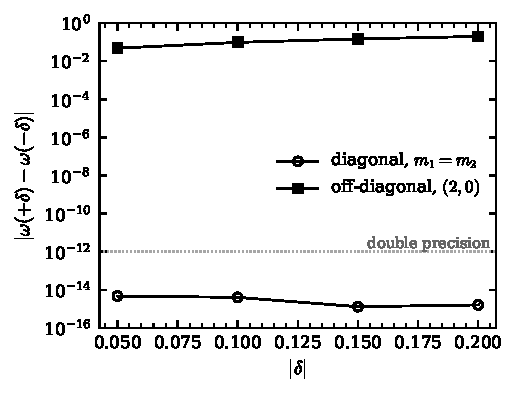
\includegraphics[width=0.62\textwidth]{figures/figS1_parity.pdf}
  \caption{Measured $\delta$-parity, $\ell=2$, $N=0$, $s=0.20$, $\mu=0.6$.}
  \label{fig:parity}
\end{figure}

%-------------------------------------------------------------------------
\section{The quasiresonant regime}\label{sec:quasi}
%-------------------------------------------------------------------------

As the scalar mass grows, branches migrate toward the threshold
$\omega^2=\mu^2$ and become arbitrarily long lived. Tracking eleven branches
across six sectors with an adaptive step in $\mu$, the damping falls through
$8.6$ orders of magnitude along a single continuous branch, from $0.357$ at
$\mu=0$ to $8.65\times10^{-10}$ at $\mu=2.968$, with $\Rem\,\omega\to\mu$
(Fig.~\ref{fig:quasi}). Each walk terminates where double precision can no
longer resolve the mode, so the minima are lower bounds on how far a branch was
followed, not infima. The transition is a branch point in $\mu$, not a
coalescence: the neighbouring overtone remains at $-\Imm\,\omega\sim0.1$
throughout.

This regime also settles a question about solver behaviour that proves to be
physics rather than numerics. Exterior complex scaling requires
$\tan\vartheta > -\Imm\,\Omega/\Rem\,\Omega$. As $\Rem\,\Omega\to0$ the outgoing
wave ceases to oscillate and the required angle tends to $90^\circ$, so no
admissible contour exists. We measure $\vartheta_{\min}=89.92^\circ$ and
$89.81^\circ$ at the two points where the recurrence-free solvers fail, against
$4.4^\circ$ at an ordinary near-extremal point where they succeed. This is a
limit of the formulation, not a convergence failure: no increase of resolution,
precision or domain decomposition removes it, which is why a multidomain
refinement of the near-horizon region did not help. It follows that the
difficulty is controlled by $\mu$, not by proximity to extremality --- ordinary
modes continue smoothly to extremality $0.0103$ with residuals $\sim10^{-13}$
over thirty-seven consecutive steps.

\begin{figure}[h]
  \centering
  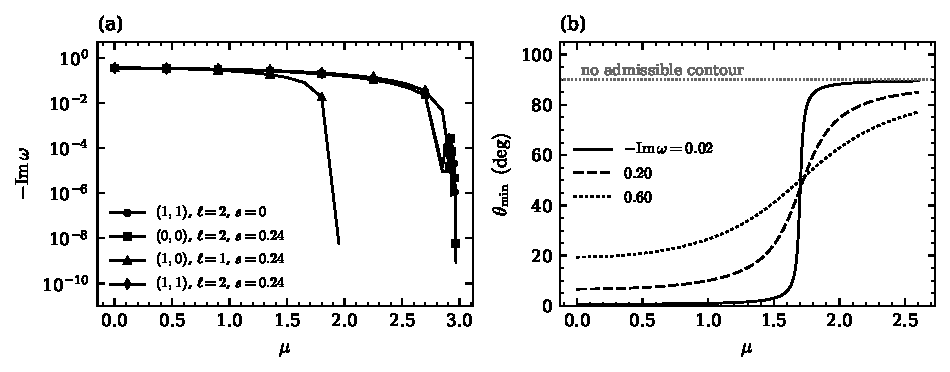
\includegraphics[width=0.96\textwidth]{figures/figS2_quasiresonance.pdf}
  \caption{(a) Damping along four branches continued in $\mu$. (b) The minimum
  admissible exterior-complex-scaling angle; as $\Rem\,\Omega\to0$ it reaches
  $90^\circ$ and the method has no admissible contour.}
  \label{fig:quasi}
\end{figure}

%-------------------------------------------------------------------------
\section{Two diagnostics withdrawn}\label{sec:withdrawn}
%-------------------------------------------------------------------------

We record two diagnostics that were used in an earlier version of this work and
are withdrawn, since both mistakes are natural and the second is subtle.

\emph{The ratio of leading Taylor coefficients.} Under $F\mapsto gF$ with $g$
holomorphic and nonvanishing, expanding about a simple root gives
$\tilde a_1=g_0a_1$ and $\tilde a_2=g_0a_2+g_1a_1$, so
$\tilde a_1/\tilde a_2=(a_1/a_2)/[1+(g_1/g_0)(a_1/a_2)]$: the ratio is only
\emph{asymptotically} insensitive to normalization, with distortion
$\Ord(|g'/g|d)$. Measured against $g=10^{7}e^{3\omega}$ the distortion follows
$|1+3d|^{-1}$ to five decimals, from $1.0003$ at $d=10^{-4}$ to $1.4286$ at
$d=0.1$. Decisively, the ratio measures the distance to the nearest zero
\emph{or pole}; Leaver's continued fraction is meromorphic, and contour
integration about the tightest candidate returns
$\mathcal{N}-\mathcal{P}=0$ at every radius out to $0.20$, so the small values
returned are pole distances.

\emph{The discriminant as independent evidence.} Since $D=(\omega_+-\omega_-)^2$,
its minimum is the square of the minimum separation --- numerically
$0.5116^2=0.26176$, agreeing to sixteen digits. It is one quantity reported
twice, and is not counted separately.

A third defect found in the course of this: the diagnostics had been evaluated
with the continued fraction inverted at index $0$ irrespective of the branch's
own overtone. The inversions are not equivalent at finite depth --- at a tracked
$N=2$ root the $N=2$ inversion gives $|F|=1.9\times10^{-13}$ while inversions
$0,1,3$ give $7\times10^{-2}$, $1\times10^{-1}$ and $1.1$, values that are
unchanged from depth $200$ to depth $3200$. A residual gate now rejects any
expansion whose constant term is not small.

%-------------------------------------------------------------------------
\section{Reproduction}\label{sec:repro}
%-------------------------------------------------------------------------

The scientific environment is locked; the plotting stack is deliberately kept
out of it so that neither the results nor continuous integration depend on a
graphics library. Verified from a fresh clone into an empty directory with a new
virtual environment.

\begin{verbatim}
  ./scripts/reproduce_core_science.sh --quick   # analytical + machinery
  ./scripts/reproduce_core_science.sh           # + atlas + collision search
  ./scripts/reproduce_full_science.sh --resume  # everything
\end{verbatim}

\end{document}
